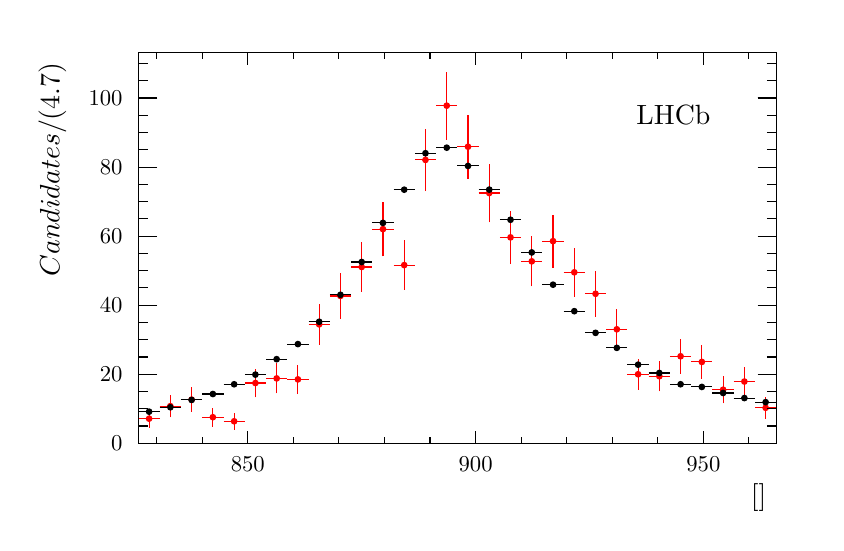
\begin{tikzpicture}
\pgfdeclareplotmark{cross} {
\pgfpathmoveto{\pgfpoint{-0.3\pgfplotmarksize}{\pgfplotmarksize}}
\pgfpathlineto{\pgfpoint{+0.3\pgfplotmarksize}{\pgfplotmarksize}}
\pgfpathlineto{\pgfpoint{+0.3\pgfplotmarksize}{0.3\pgfplotmarksize}}
\pgfpathlineto{\pgfpoint{+1\pgfplotmarksize}{0.3\pgfplotmarksize}}
\pgfpathlineto{\pgfpoint{+1\pgfplotmarksize}{-0.3\pgfplotmarksize}}
\pgfpathlineto{\pgfpoint{+0.3\pgfplotmarksize}{-0.3\pgfplotmarksize}}
\pgfpathlineto{\pgfpoint{+0.3\pgfplotmarksize}{-1.\pgfplotmarksize}}
\pgfpathlineto{\pgfpoint{-0.3\pgfplotmarksize}{-1.\pgfplotmarksize}}
\pgfpathlineto{\pgfpoint{-0.3\pgfplotmarksize}{-0.3\pgfplotmarksize}}
\pgfpathlineto{\pgfpoint{-1.\pgfplotmarksize}{-0.3\pgfplotmarksize}}
\pgfpathlineto{\pgfpoint{-1.\pgfplotmarksize}{0.3\pgfplotmarksize}}
\pgfpathlineto{\pgfpoint{-0.3\pgfplotmarksize}{0.3\pgfplotmarksize}}
\pgfpathclose
\pgfusepathqstroke
}
\pgfdeclareplotmark{cross*} {
\pgfpathmoveto{\pgfpoint{-0.3\pgfplotmarksize}{\pgfplotmarksize}}
\pgfpathlineto{\pgfpoint{+0.3\pgfplotmarksize}{\pgfplotmarksize}}
\pgfpathlineto{\pgfpoint{+0.3\pgfplotmarksize}{0.3\pgfplotmarksize}}
\pgfpathlineto{\pgfpoint{+1\pgfplotmarksize}{0.3\pgfplotmarksize}}
\pgfpathlineto{\pgfpoint{+1\pgfplotmarksize}{-0.3\pgfplotmarksize}}
\pgfpathlineto{\pgfpoint{+0.3\pgfplotmarksize}{-0.3\pgfplotmarksize}}
\pgfpathlineto{\pgfpoint{+0.3\pgfplotmarksize}{-1.\pgfplotmarksize}}
\pgfpathlineto{\pgfpoint{-0.3\pgfplotmarksize}{-1.\pgfplotmarksize}}
\pgfpathlineto{\pgfpoint{-0.3\pgfplotmarksize}{-0.3\pgfplotmarksize}}
\pgfpathlineto{\pgfpoint{-1.\pgfplotmarksize}{-0.3\pgfplotmarksize}}
\pgfpathlineto{\pgfpoint{-1.\pgfplotmarksize}{0.3\pgfplotmarksize}}
\pgfpathlineto{\pgfpoint{-0.3\pgfplotmarksize}{0.3\pgfplotmarksize}}
\pgfpathclose
\pgfusepathqfillstroke
}
\pgfdeclareplotmark{newstar} {
\pgfpathmoveto{\pgfqpoint{0pt}{\pgfplotmarksize}}
\pgfpathlineto{\pgfqpointpolar{44}{0.5\pgfplotmarksize}}
\pgfpathlineto{\pgfqpointpolar{18}{\pgfplotmarksize}}
\pgfpathlineto{\pgfqpointpolar{-20}{0.5\pgfplotmarksize}}
\pgfpathlineto{\pgfqpointpolar{-54}{\pgfplotmarksize}}
\pgfpathlineto{\pgfqpointpolar{-90}{0.5\pgfplotmarksize}}
\pgfpathlineto{\pgfqpointpolar{234}{\pgfplotmarksize}}
\pgfpathlineto{\pgfqpointpolar{198}{0.5\pgfplotmarksize}}
\pgfpathlineto{\pgfqpointpolar{162}{\pgfplotmarksize}}
\pgfpathlineto{\pgfqpointpolar{134}{0.5\pgfplotmarksize}}
\pgfpathclose
\pgfusepathqstroke
}
\pgfdeclareplotmark{newstar*} {
\pgfpathmoveto{\pgfqpoint{0pt}{\pgfplotmarksize}}
\pgfpathlineto{\pgfqpointpolar{44}{0.5\pgfplotmarksize}}
\pgfpathlineto{\pgfqpointpolar{18}{\pgfplotmarksize}}
\pgfpathlineto{\pgfqpointpolar{-20}{0.5\pgfplotmarksize}}
\pgfpathlineto{\pgfqpointpolar{-54}{\pgfplotmarksize}}
\pgfpathlineto{\pgfqpointpolar{-90}{0.5\pgfplotmarksize}}
\pgfpathlineto{\pgfqpointpolar{234}{\pgfplotmarksize}}
\pgfpathlineto{\pgfqpointpolar{198}{0.5\pgfplotmarksize}}
\pgfpathlineto{\pgfqpointpolar{162}{\pgfplotmarksize}}
\pgfpathlineto{\pgfqpointpolar{134}{0.5\pgfplotmarksize}}
\pgfpathclose
\pgfusepathqfillstroke
}
\definecolor{c}{rgb}{1,1,1};
\draw [color=c, fill=c] (0,0) rectangle (10,6.27517);
\draw [color=c, fill=c] (1.4,1.00403) rectangle (9.5,5.96141);
\definecolor{c}{rgb}{0,0,0};
\draw [c] (1.4,1.00403) -- (1.4,5.96141) -- (9.5,5.96141) -- (9.5,1.00403) -- (1.4,1.00403);
\definecolor{c}{rgb}{1,1,1};
\draw [color=c, fill=c] (1.4,1.00403) rectangle (9.5,5.96141);
\definecolor{c}{rgb}{0,0,0};
\draw [c] (1.4,1.00403) -- (1.4,5.96141) -- (9.5,5.96141) -- (9.5,1.00403) -- (1.4,1.00403);
\definecolor{c}{rgb}{1,0,0};
\draw [c,line width=0.4] (1.535,1.19957) -- (1.535,1.31664);
\draw [c,line width=0.4] (1.535,1.31664) -- (1.535,1.43372);
\draw [c,line width=0.4] (1.4,1.31664) -- (1.535,1.31664);
\draw [c,line width=0.4] (1.535,1.31664) -- (1.67,1.31664);
\foreach \P in {(1.535,1.31664)}{\draw[mark options={color=c,fill=c},mark size=2.402402pt,mark=*,mark size=1pt] plot coordinates {\P};}
\draw [c,line width=0.4] (1.805,1.33205) -- (1.805,1.47588);
\draw [c,line width=0.4] (1.805,1.47588) -- (1.805,1.61971);
\draw [c,line width=0.4] (1.67,1.47588) -- (1.805,1.47588);
\draw [c,line width=0.4] (1.805,1.47588) -- (1.94,1.47588);
\foreach \P in {(1.805,1.47588)}{\draw[mark options={color=c,fill=c},mark size=2.402402pt,mark=*,mark size=1pt] plot coordinates {\P};}
\draw [c,line width=0.4] (2.075,1.40272) -- (2.075,1.55866);
\draw [c,line width=0.4] (2.075,1.55866) -- (2.075,1.7146);
\draw [c,line width=0.4] (1.94,1.55866) -- (2.075,1.55866);
\draw [c,line width=0.4] (2.075,1.55866) -- (2.21,1.55866);
\foreach \P in {(2.075,1.55866)}{\draw[mark options={color=c,fill=c},mark size=2.402402pt,mark=*,mark size=1pt] plot coordinates {\P};}
\draw [c,line width=0.4] (2.345,1.21472) -- (2.345,1.33522);
\draw [c,line width=0.4] (2.345,1.33522) -- (2.345,1.45572);
\draw [c,line width=0.4] (2.21,1.33522) -- (2.345,1.33522);
\draw [c,line width=0.4] (2.345,1.33522) -- (2.48,1.33522);
\foreach \P in {(2.345,1.33522)}{\draw[mark options={color=c,fill=c},mark size=2.402402pt,mark=*,mark size=1pt] plot coordinates {\P};}
\draw [c,line width=0.4] (2.615,1.1728) -- (2.615,1.28349);
\draw [c,line width=0.4] (2.615,1.28349) -- (2.615,1.39418);
\draw [c,line width=0.4] (2.48,1.28349) -- (2.615,1.28349);
\draw [c,line width=0.4] (2.615,1.28349) -- (2.75,1.28349);
\foreach \P in {(2.615,1.28349)}{\draw[mark options={color=c,fill=c},mark size=2.402402pt,mark=*,mark size=1pt] plot coordinates {\P};}
\draw [c,line width=0.4] (2.885,1.58588) -- (2.885,1.76902);
\draw [c,line width=0.4] (2.885,1.76902) -- (2.885,1.95217);
\draw [c,line width=0.4] (2.75,1.76902) -- (2.885,1.76902);
\draw [c,line width=0.4] (2.885,1.76902) -- (3.02,1.76902);
\foreach \P in {(2.885,1.76902)}{\draw[mark options={color=c,fill=c},mark size=2.402402pt,mark=*,mark size=1pt] plot coordinates {\P};}
\draw [c,line width=0.4] (3.155,1.63803) -- (3.155,1.82811);
\draw [c,line width=0.4] (3.155,1.82811) -- (3.155,2.01819);
\draw [c,line width=0.4] (3.02,1.82811) -- (3.155,1.82811);
\draw [c,line width=0.4] (3.155,1.82811) -- (3.29,1.82811);
\foreach \P in {(3.155,1.82811)}{\draw[mark options={color=c,fill=c},mark size=2.402402pt,mark=*,mark size=1pt] plot coordinates {\P};}
\draw [c,line width=0.4] (3.425,1.6269) -- (3.425,1.81553);
\draw [c,line width=0.4] (3.425,1.81553) -- (3.425,2.00415);
\draw [c,line width=0.4] (3.29,1.81553) -- (3.425,1.81553);
\draw [c,line width=0.4] (3.425,1.81553) -- (3.56,1.81553);
\foreach \P in {(3.425,1.81553)}{\draw[mark options={color=c,fill=c},mark size=2.402402pt,mark=*,mark size=1pt] plot coordinates {\P};}
\draw [c,line width=0.4] (3.695,2.25727) -- (3.695,2.51463);
\draw [c,line width=0.4] (3.695,2.51463) -- (3.695,2.77198);
\draw [c,line width=0.4] (3.56,2.51463) -- (3.695,2.51463);
\draw [c,line width=0.4] (3.695,2.51463) -- (3.83,2.51463);
\foreach \P in {(3.695,2.51463)}{\draw[mark options={color=c,fill=c},mark size=2.402402pt,mark=*,mark size=1pt] plot coordinates {\P};}
\draw [c,line width=0.4] (3.965,2.58844) -- (3.965,2.87484);
\draw [c,line width=0.4] (3.965,2.87484) -- (3.965,3.16123);
\draw [c,line width=0.4] (3.83,2.87484) -- (3.965,2.87484);
\draw [c,line width=0.4] (3.965,2.87484) -- (4.1,2.87484);
\foreach \P in {(3.965,2.87484)}{\draw[mark options={color=c,fill=c},mark size=2.402402pt,mark=*,mark size=1pt] plot coordinates {\P};}
\draw [c,line width=0.4] (4.235,2.92954) -- (4.235,3.24284);
\draw [c,line width=0.4] (4.235,3.24284) -- (4.235,3.55614);
\draw [c,line width=0.4] (4.1,3.24284) -- (4.235,3.24284);
\draw [c,line width=0.4] (4.235,3.24284) -- (4.37,3.24284);
\foreach \P in {(4.235,3.24284)}{\draw[mark options={color=c,fill=c},mark size=2.402402pt,mark=*,mark size=1pt] plot coordinates {\P};}
\draw [c,line width=0.4] (4.505,3.37847) -- (4.505,3.72379);
\draw [c,line width=0.4] (4.505,3.72379) -- (4.505,4.0691);
\draw [c,line width=0.4] (4.37,3.72379) -- (4.505,3.72379);
\draw [c,line width=0.4] (4.505,3.72379) -- (4.64,3.72379);
\foreach \P in {(4.505,3.72379)}{\draw[mark options={color=c,fill=c},mark size=2.402402pt,mark=*,mark size=1pt] plot coordinates {\P};}
\draw [c,line width=0.4] (4.775,2.95201) -- (4.775,3.267);
\draw [c,line width=0.4] (4.775,3.267) -- (4.775,3.58199);
\draw [c,line width=0.4] (4.64,3.267) -- (4.775,3.267);
\draw [c,line width=0.4] (4.775,3.267) -- (4.91,3.267);
\foreach \P in {(4.775,3.267)}{\draw[mark options={color=c,fill=c},mark size=2.402402pt,mark=*,mark size=1pt] plot coordinates {\P};}
\draw [c,line width=0.4] (5.045,4.20541) -- (5.045,4.60262);
\draw [c,line width=0.4] (5.045,4.60262) -- (5.045,4.99983);
\draw [c,line width=0.4] (4.91,4.60262) -- (5.045,4.60262);
\draw [c,line width=0.4] (5.045,4.60262) -- (5.18,4.60262);
\foreach \P in {(5.045,4.60262)}{\draw[mark options={color=c,fill=c},mark size=2.402402pt,mark=*,mark size=1pt] plot coordinates {\P};}
\draw [c,line width=0.4] (5.315,4.85819) -- (5.315,5.29177);
\draw [c,line width=0.4] (5.315,5.29177) -- (5.315,5.72534);
\draw [c,line width=0.4] (5.18,5.29177) -- (5.315,5.29177);
\draw [c,line width=0.4] (5.315,5.29177) -- (5.45,5.29177);
\foreach \P in {(5.315,5.29177)}{\draw[mark options={color=c,fill=c},mark size=2.402402pt,mark=*,mark size=1pt] plot coordinates {\P};}
\draw [c,line width=0.4] (5.585,4.36369) -- (5.585,4.77003);
\draw [c,line width=0.4] (5.585,4.77003) -- (5.585,5.17637);
\draw [c,line width=0.4] (5.45,4.77003) -- (5.585,4.77003);
\draw [c,line width=0.4] (5.585,4.77003) -- (5.72,4.77003);
\foreach \P in {(5.585,4.77003)}{\draw[mark options={color=c,fill=c},mark size=2.402402pt,mark=*,mark size=1pt] plot coordinates {\P};}
\draw [c,line width=0.4] (5.855,3.80857) -- (5.855,4.18184);
\draw [c,line width=0.4] (5.855,4.18184) -- (5.855,4.5551);
\draw [c,line width=0.4] (5.72,4.18184) -- (5.855,4.18184);
\draw [c,line width=0.4] (5.855,4.18184) -- (5.99,4.18184);
\foreach \P in {(5.855,4.18184)}{\draw[mark options={color=c,fill=c},mark size=2.402402pt,mark=*,mark size=1pt] plot coordinates {\P};}
\draw [c,line width=0.4] (6.125,3.28046) -- (6.125,3.61906);
\draw [c,line width=0.4] (6.125,3.61906) -- (6.125,3.95767);
\draw [c,line width=0.4] (5.99,3.61906) -- (6.125,3.61906);
\draw [c,line width=0.4] (6.125,3.61906) -- (6.26,3.61906);
\foreach \P in {(6.125,3.61906)}{\draw[mark options={color=c,fill=c},mark size=2.402402pt,mark=*,mark size=1pt] plot coordinates {\P};}
\draw [c,line width=0.4] (6.395,2.99647) -- (6.395,3.31476);
\draw [c,line width=0.4] (6.395,3.31476) -- (6.395,3.63305);
\draw [c,line width=0.4] (6.26,3.31476) -- (6.395,3.31476);
\draw [c,line width=0.4] (6.395,3.31476) -- (6.53,3.31476);
\foreach \P in {(6.395,3.31476)}{\draw[mark options={color=c,fill=c},mark size=2.402402pt,mark=*,mark size=1pt] plot coordinates {\P};}
\draw [c,line width=0.4] (6.665,3.23579) -- (6.665,3.57129);
\draw [c,line width=0.4] (6.665,3.57129) -- (6.665,3.90678);
\draw [c,line width=0.4] (6.53,3.57129) -- (6.665,3.57129);
\draw [c,line width=0.4] (6.665,3.57129) -- (6.8,3.57129);
\foreach \P in {(6.665,3.57129)}{\draw[mark options={color=c,fill=c},mark size=2.402402pt,mark=*,mark size=1pt] plot coordinates {\P};}
\draw [c,line width=0.4] (6.935,2.86697) -- (6.935,3.17553);
\draw [c,line width=0.4] (6.935,3.17553) -- (6.935,3.48409);
\draw [c,line width=0.4] (6.8,3.17553) -- (6.935,3.17553);
\draw [c,line width=0.4] (6.935,3.17553) -- (7.07,3.17553);
\foreach \P in {(6.935,3.17553)}{\draw[mark options={color=c,fill=c},mark size=2.402402pt,mark=*,mark size=1pt] plot coordinates {\P};}
\draw [c,line width=0.4] (7.205,2.61382) -- (7.205,2.90231);
\draw [c,line width=0.4] (7.205,2.90231) -- (7.205,3.1908);
\draw [c,line width=0.4] (7.07,2.90231) -- (7.205,2.90231);
\draw [c,line width=0.4] (7.205,2.90231) -- (7.34,2.90231);
\foreach \P in {(7.205,2.90231)}{\draw[mark options={color=c,fill=c},mark size=2.402402pt,mark=*,mark size=1pt] plot coordinates {\P};}
\draw [c,line width=0.4] (7.475,2.19965) -- (7.475,2.45158);
\draw [c,line width=0.4] (7.475,2.45158) -- (7.475,2.7035);
\draw [c,line width=0.4] (7.34,2.45158) -- (7.475,2.45158);
\draw [c,line width=0.4] (7.475,2.45158) -- (7.61,2.45158);
\foreach \P in {(7.475,2.45158)}{\draw[mark options={color=c,fill=c},mark size=2.402402pt,mark=*,mark size=1pt] plot coordinates {\P};}
\draw [c,line width=0.4] (7.745,1.68472) -- (7.745,1.88078);
\draw [c,line width=0.4] (7.745,1.88078) -- (7.745,2.07684);
\draw [c,line width=0.4] (7.61,1.88078) -- (7.745,1.88078);
\draw [c,line width=0.4] (7.745,1.88078) -- (7.88,1.88078);
\foreach \P in {(7.745,1.88078)}{\draw[mark options={color=c,fill=c},mark size=2.402402pt,mark=*,mark size=1pt] plot coordinates {\P};}
\draw [c,line width=0.4] (8.015,1.66236) -- (8.015,1.85558);
\draw [c,line width=0.4] (8.015,1.85558) -- (8.015,2.04881);
\draw [c,line width=0.4] (7.88,1.85558) -- (8.015,1.85558);
\draw [c,line width=0.4] (8.015,1.85558) -- (8.15,1.85558);
\foreach \P in {(8.015,1.85558)}{\draw[mark options={color=c,fill=c},mark size=2.402402pt,mark=*,mark size=1pt] plot coordinates {\P};}
\draw [c,line width=0.4] (8.285,1.88881) -- (8.285,2.1089);
\draw [c,line width=0.4] (8.285,2.1089) -- (8.285,2.329);
\draw [c,line width=0.4] (8.15,2.1089) -- (8.285,2.1089);
\draw [c,line width=0.4] (8.285,2.1089) -- (8.42,2.1089);
\foreach \P in {(8.285,2.1089)}{\draw[mark options={color=c,fill=c},mark size=2.402402pt,mark=*,mark size=1pt] plot coordinates {\P};}
\draw [c,line width=0.4] (8.555,1.82438) -- (8.555,2.03721);
\draw [c,line width=0.4] (8.555,2.03721) -- (8.555,2.25005);
\draw [c,line width=0.4] (8.42,2.03721) -- (8.555,2.03721);
\draw [c,line width=0.4] (8.555,2.03721) -- (8.69,2.03721);
\foreach \P in {(8.555,2.03721)}{\draw[mark options={color=c,fill=c},mark size=2.402402pt,mark=*,mark size=1pt] plot coordinates {\P};}
\draw [c,line width=0.4] (8.825,1.51149) -- (8.825,1.68417);
\draw [c,line width=0.4] (8.825,1.68417) -- (8.825,1.85685);
\draw [c,line width=0.4] (8.69,1.68417) -- (8.825,1.68417);
\draw [c,line width=0.4] (8.825,1.68417) -- (8.96,1.68417);
\foreach \P in {(8.825,1.68417)}{\draw[mark options={color=c,fill=c},mark size=2.402402pt,mark=*,mark size=1pt] plot coordinates {\P};}
\draw [c,line width=0.4] (9.095,1.60294) -- (9.095,1.78839);
\draw [c,line width=0.4] (9.095,1.78839) -- (9.095,1.97383);
\draw [c,line width=0.4] (8.96,1.78839) -- (9.095,1.78839);
\draw [c,line width=0.4] (9.095,1.78839) -- (9.23,1.78839);
\foreach \P in {(9.095,1.78839)}{\draw[mark options={color=c,fill=c},mark size=2.402402pt,mark=*,mark size=1pt] plot coordinates {\P};}
\draw [c,line width=0.4] (9.365,1.31423) -- (9.365,1.45481);
\draw [c,line width=0.4] (9.365,1.45481) -- (9.365,1.5954);
\draw [c,line width=0.4] (9.23,1.45481) -- (9.365,1.45481);
\draw [c,line width=0.4] (9.365,1.45481) -- (9.5,1.45481);
\foreach \P in {(9.365,1.45481)}{\draw[mark options={color=c,fill=c},mark size=2.402402pt,mark=*,mark size=1pt] plot coordinates {\P};}
\definecolor{c}{rgb}{0,0,0};
\draw [c,line width=0.4] (1.4,1.00403) -- (9.5,1.00403);
\draw [anchor= east] (9.5,0.317272) node[scale=1.00614, rotate=0]{$\mkpi [\mevcc]$};
\draw [c,line width=0.4] (2.78857,1.15651) -- (2.78857,1.00403);
\draw [c,line width=0.4] (3.36714,1.08027) -- (3.36714,1.00403);
\draw [c,line width=0.4] (3.94571,1.08027) -- (3.94571,1.00403);
\draw [c,line width=0.4] (4.52429,1.08027) -- (4.52429,1.00403);
\draw [c,line width=0.4] (5.10286,1.08027) -- (5.10286,1.00403);
\draw [c,line width=0.4] (5.68143,1.15651) -- (5.68143,1.00403);
\draw [c,line width=0.4] (6.26,1.08027) -- (6.26,1.00403);
\draw [c,line width=0.4] (6.83857,1.08027) -- (6.83857,1.00403);
\draw [c,line width=0.4] (7.41714,1.08027) -- (7.41714,1.00403);
\draw [c,line width=0.4] (7.99571,1.08027) -- (7.99571,1.00403);
\draw [c,line width=0.4] (8.57429,1.15651) -- (8.57429,1.00403);
\draw [c,line width=0.4] (2.78857,1.15651) -- (2.78857,1.00403);
\draw [c,line width=0.4] (2.21,1.08027) -- (2.21,1.00403);
\draw [c,line width=0.4] (1.63143,1.08027) -- (1.63143,1.00403);
\draw [c,line width=0.4] (8.57429,1.15651) -- (8.57429,1.00403);
\draw [c,line width=0.4] (9.15286,1.08027) -- (9.15286,1.00403);
\draw [anchor=base] (2.78857,0.640067) node[scale=0.819821, rotate=0]{850};
\draw [anchor=base] (5.68143,0.640067) node[scale=0.819821, rotate=0]{900};
\draw [anchor=base] (8.57429,0.640067) node[scale=0.819821, rotate=0]{950};
\draw [c,line width=0.4] (1.4,5.96141) -- (9.5,5.96141);
\draw [c,line width=0.4] (2.78857,5.80892) -- (2.78857,5.96141);
\draw [c,line width=0.4] (3.36714,5.88517) -- (3.36714,5.96141);
\draw [c,line width=0.4] (3.94571,5.88517) -- (3.94571,5.96141);
\draw [c,line width=0.4] (4.52429,5.88517) -- (4.52429,5.96141);
\draw [c,line width=0.4] (5.10286,5.88517) -- (5.10286,5.96141);
\draw [c,line width=0.4] (5.68143,5.80892) -- (5.68143,5.96141);
\draw [c,line width=0.4] (6.26,5.88517) -- (6.26,5.96141);
\draw [c,line width=0.4] (6.83857,5.88517) -- (6.83857,5.96141);
\draw [c,line width=0.4] (7.41714,5.88517) -- (7.41714,5.96141);
\draw [c,line width=0.4] (7.99571,5.88517) -- (7.99571,5.96141);
\draw [c,line width=0.4] (8.57429,5.80892) -- (8.57429,5.96141);
\draw [c,line width=0.4] (2.78857,5.80892) -- (2.78857,5.96141);
\draw [c,line width=0.4] (2.21,5.88517) -- (2.21,5.96141);
\draw [c,line width=0.4] (1.63143,5.88517) -- (1.63143,5.96141);
\draw [c,line width=0.4] (8.57429,5.80892) -- (8.57429,5.96141);
\draw [c,line width=0.4] (9.15286,5.88517) -- (9.15286,5.96141);
\draw [c,line width=0.4] (1.4,1.00403) -- (1.4,5.96141);
\draw [anchor= east] (0.3056,5.96141) node[scale=1.00614, rotate=90]{$\text{Candidates} / (4.7 \mevcc)$};
\draw [c,line width=0.4] (1.637,1.00403) -- (1.4,1.00403);
\draw [c,line width=0.4] (1.5185,1.22325) -- (1.4,1.22325);
\draw [c,line width=0.4] (1.5185,1.44246) -- (1.4,1.44246);
\draw [c,line width=0.4] (1.5185,1.66168) -- (1.4,1.66168);
\draw [c,line width=0.4] (1.637,1.8809) -- (1.4,1.8809);
\draw [c,line width=0.4] (1.5185,2.10012) -- (1.4,2.10012);
\draw [c,line width=0.4] (1.5185,2.31934) -- (1.4,2.31934);
\draw [c,line width=0.4] (1.5185,2.53855) -- (1.4,2.53855);
\draw [c,line width=0.4] (1.637,2.75777) -- (1.4,2.75777);
\draw [c,line width=0.4] (1.5185,2.97699) -- (1.4,2.97699);
\draw [c,line width=0.4] (1.5185,3.19621) -- (1.4,3.19621);
\draw [c,line width=0.4] (1.5185,3.41543) -- (1.4,3.41543);
\draw [c,line width=0.4] (1.637,3.63465) -- (1.4,3.63465);
\draw [c,line width=0.4] (1.5185,3.85386) -- (1.4,3.85386);
\draw [c,line width=0.4] (1.5185,4.07308) -- (1.4,4.07308);
\draw [c,line width=0.4] (1.5185,4.2923) -- (1.4,4.2923);
\draw [c,line width=0.4] (1.637,4.51152) -- (1.4,4.51152);
\draw [c,line width=0.4] (1.5185,4.73074) -- (1.4,4.73074);
\draw [c,line width=0.4] (1.5185,4.94996) -- (1.4,4.94996);
\draw [c,line width=0.4] (1.5185,5.16917) -- (1.4,5.16917);
\draw [c,line width=0.4] (1.637,5.38839) -- (1.4,5.38839);
\draw [c,line width=0.4] (1.637,5.38839) -- (1.4,5.38839);
\draw [c,line width=0.4] (1.5185,5.60761) -- (1.4,5.60761);
\draw [c,line width=0.4] (1.5185,5.82683) -- (1.4,5.82683);
\draw [anchor= east] (1.3,1.00403) node[scale=0.819821, rotate=0]{0};
\draw [anchor= east] (1.3,1.8809) node[scale=0.819821, rotate=0]{20};
\draw [anchor= east] (1.3,2.75777) node[scale=0.819821, rotate=0]{40};
\draw [anchor= east] (1.3,3.63465) node[scale=0.819821, rotate=0]{60};
\draw [anchor= east] (1.3,4.51152) node[scale=0.819821, rotate=0]{80};
\draw [anchor= east] (1.3,5.38839) node[scale=0.819821, rotate=0]{100};
\draw [c,line width=0.4] (9.5,1.00403) -- (9.5,5.96141);
\draw [c,line width=0.4] (9.263,1.00403) -- (9.5,1.00403);
\draw [c,line width=0.4] (9.3815,1.22325) -- (9.5,1.22325);
\draw [c,line width=0.4] (9.3815,1.44246) -- (9.5,1.44246);
\draw [c,line width=0.4] (9.3815,1.66168) -- (9.5,1.66168);
\draw [c,line width=0.4] (9.263,1.8809) -- (9.5,1.8809);
\draw [c,line width=0.4] (9.3815,2.10012) -- (9.5,2.10012);
\draw [c,line width=0.4] (9.3815,2.31934) -- (9.5,2.31934);
\draw [c,line width=0.4] (9.3815,2.53855) -- (9.5,2.53855);
\draw [c,line width=0.4] (9.263,2.75777) -- (9.5,2.75777);
\draw [c,line width=0.4] (9.3815,2.97699) -- (9.5,2.97699);
\draw [c,line width=0.4] (9.3815,3.19621) -- (9.5,3.19621);
\draw [c,line width=0.4] (9.3815,3.41543) -- (9.5,3.41543);
\draw [c,line width=0.4] (9.263,3.63465) -- (9.5,3.63465);
\draw [c,line width=0.4] (9.3815,3.85386) -- (9.5,3.85386);
\draw [c,line width=0.4] (9.3815,4.07308) -- (9.5,4.07308);
\draw [c,line width=0.4] (9.3815,4.2923) -- (9.5,4.2923);
\draw [c,line width=0.4] (9.263,4.51152) -- (9.5,4.51152);
\draw [c,line width=0.4] (9.3815,4.73074) -- (9.5,4.73074);
\draw [c,line width=0.4] (9.3815,4.94996) -- (9.5,4.94996);
\draw [c,line width=0.4] (9.3815,5.16917) -- (9.5,5.16917);
\draw [c,line width=0.4] (9.263,5.38839) -- (9.5,5.38839);
\draw [c,line width=0.4] (9.263,5.38839) -- (9.5,5.38839);
\draw [c,line width=0.4] (9.3815,5.60761) -- (9.5,5.60761);
\draw [c,line width=0.4] (9.3815,5.82683) -- (9.5,5.82683);
\draw [c,line width=0.4] (1.535,1.39507) -- (1.535,1.40544);
\draw [c,line width=0.4] (1.535,1.40544) -- (1.535,1.41581);
\draw [c,line width=0.4] (1.4,1.40544) -- (1.535,1.40544);
\draw [c,line width=0.4] (1.535,1.40544) -- (1.67,1.40544);
\foreach \P in {(1.535,1.40544)}{\draw[mark options={color=c,fill=c},mark size=2.402402pt,mark=*,mark size=1pt] plot coordinates {\P};}
\draw [c,line width=0.4] (1.805,1.45033) -- (1.805,1.4614);
\draw [c,line width=0.4] (1.805,1.4614) -- (1.805,1.47247);
\draw [c,line width=0.4] (1.67,1.4614) -- (1.805,1.4614);
\draw [c,line width=0.4] (1.805,1.4614) -- (1.94,1.4614);
\foreach \P in {(1.805,1.4614)}{\draw[mark options={color=c,fill=c},mark size=2.402402pt,mark=*,mark size=1pt] plot coordinates {\P};}
\draw [c,line width=0.4] (2.075,1.54259) -- (2.075,1.55473);
\draw [c,line width=0.4] (2.075,1.55473) -- (2.075,1.56688);
\draw [c,line width=0.4] (1.94,1.55473) -- (2.075,1.55473);
\draw [c,line width=0.4] (2.075,1.55473) -- (2.21,1.55473);
\foreach \P in {(2.075,1.55473)}{\draw[mark options={color=c,fill=c},mark size=2.402402pt,mark=*,mark size=1pt] plot coordinates {\P};}
\draw [c,line width=0.4] (2.345,1.61643) -- (2.345,1.62937);
\draw [c,line width=0.4] (2.345,1.62937) -- (2.345,1.64231);
\draw [c,line width=0.4] (2.21,1.62937) -- (2.345,1.62937);
\draw [c,line width=0.4] (2.345,1.62937) -- (2.48,1.62937);
\foreach \P in {(2.345,1.62937)}{\draw[mark options={color=c,fill=c},mark size=2.402402pt,mark=*,mark size=1pt] plot coordinates {\P};}
\draw [c,line width=0.4] (2.615,1.73925) -- (2.615,1.75342);
\draw [c,line width=0.4] (2.615,1.75342) -- (2.615,1.76759);
\draw [c,line width=0.4] (2.48,1.75342) -- (2.615,1.75342);
\draw [c,line width=0.4] (2.615,1.75342) -- (2.75,1.75342);
\foreach \P in {(2.615,1.75342)}{\draw[mark options={color=c,fill=c},mark size=2.402402pt,mark=*,mark size=1pt] plot coordinates {\P};}
\draw [c,line width=0.4] (2.885,1.86083) -- (2.885,1.87611);
\draw [c,line width=0.4] (2.885,1.87611) -- (2.885,1.8914);
\draw [c,line width=0.4] (2.75,1.87611) -- (2.885,1.87611);
\draw [c,line width=0.4] (2.885,1.87611) -- (3.02,1.87611);
\foreach \P in {(2.885,1.87611)}{\draw[mark options={color=c,fill=c},mark size=2.402402pt,mark=*,mark size=1pt] plot coordinates {\P};}
\draw [c,line width=0.4] (3.155,2.05515) -- (3.155,2.07207);
\draw [c,line width=0.4] (3.155,2.07207) -- (3.155,2.08898);
\draw [c,line width=0.4] (3.02,2.07207) -- (3.155,2.07207);
\draw [c,line width=0.4] (3.155,2.07207) -- (3.29,2.07207);
\foreach \P in {(3.155,2.07207)}{\draw[mark options={color=c,fill=c},mark size=2.402402pt,mark=*,mark size=1pt] plot coordinates {\P};}
\draw [c,line width=0.4] (3.425,2.24542) -- (3.425,2.26379);
\draw [c,line width=0.4] (3.425,2.26379) -- (3.425,2.28216);
\draw [c,line width=0.4] (3.29,2.26379) -- (3.425,2.26379);
\draw [c,line width=0.4] (3.425,2.26379) -- (3.56,2.26379);
\foreach \P in {(3.425,2.26379)}{\draw[mark options={color=c,fill=c},mark size=2.402402pt,mark=*,mark size=1pt] plot coordinates {\P};}
\draw [c,line width=0.4] (3.695,2.52726) -- (3.695,2.54759);
\draw [c,line width=0.4] (3.695,2.54759) -- (3.695,2.56792);
\draw [c,line width=0.4] (3.56,2.54759) -- (3.695,2.54759);
\draw [c,line width=0.4] (3.695,2.54759) -- (3.83,2.54759);
\foreach \P in {(3.695,2.54759)}{\draw[mark options={color=c,fill=c},mark size=2.402402pt,mark=*,mark size=1pt] plot coordinates {\P};}
\draw [c,line width=0.4] (3.965,2.867) -- (3.965,2.88947);
\draw [c,line width=0.4] (3.965,2.88947) -- (3.965,2.91194);
\draw [c,line width=0.4] (3.83,2.88947) -- (3.965,2.88947);
\draw [c,line width=0.4] (3.965,2.88947) -- (4.1,2.88947);
\foreach \P in {(3.965,2.88947)}{\draw[mark options={color=c,fill=c},mark size=2.402402pt,mark=*,mark size=1pt] plot coordinates {\P};}
\draw [c,line width=0.4] (4.235,3.28129) -- (4.235,3.30612);
\draw [c,line width=0.4] (4.235,3.30612) -- (4.235,3.33096);
\draw [c,line width=0.4] (4.1,3.30612) -- (4.235,3.30612);
\draw [c,line width=0.4] (4.235,3.30612) -- (4.37,3.30612);
\foreach \P in {(4.235,3.30612)}{\draw[mark options={color=c,fill=c},mark size=2.402402pt,mark=*,mark size=1pt] plot coordinates {\P};}
\draw [c,line width=0.4] (4.505,3.77529) -- (4.505,3.80267);
\draw [c,line width=0.4] (4.505,3.80267) -- (4.505,3.83004);
\draw [c,line width=0.4] (4.37,3.80267) -- (4.505,3.80267);
\draw [c,line width=0.4] (4.505,3.80267) -- (4.64,3.80267);
\foreach \P in {(4.505,3.80267)}{\draw[mark options={color=c,fill=c},mark size=2.402402pt,mark=*,mark size=1pt] plot coordinates {\P};}
\draw [c,line width=0.4] (4.775,4.1951) -- (4.775,4.22447);
\draw [c,line width=0.4] (4.775,4.22447) -- (4.775,4.25384);
\draw [c,line width=0.4] (4.64,4.22447) -- (4.775,4.22447);
\draw [c,line width=0.4] (4.775,4.22447) -- (4.91,4.22447);
\foreach \P in {(4.775,4.22447)}{\draw[mark options={color=c,fill=c},mark size=2.402402pt,mark=*,mark size=1pt] plot coordinates {\P};}
\draw [c,line width=0.4] (5.045,4.65623) -- (5.045,4.68764);
\draw [c,line width=0.4] (5.045,4.68764) -- (5.045,4.71905);
\draw [c,line width=0.4] (4.91,4.68764) -- (5.045,4.68764);
\draw [c,line width=0.4] (5.045,4.68764) -- (5.18,4.68764);
\foreach \P in {(5.045,4.68764)}{\draw[mark options={color=c,fill=c},mark size=2.402402pt,mark=*,mark size=1pt] plot coordinates {\P};}
\draw [c,line width=0.4] (5.315,4.72635) -- (5.315,4.75805);
\draw [c,line width=0.4] (5.315,4.75805) -- (5.315,4.78976);
\draw [c,line width=0.4] (5.18,4.75805) -- (5.315,4.75805);
\draw [c,line width=0.4] (5.315,4.75805) -- (5.45,4.75805);
\foreach \P in {(5.315,4.75805)}{\draw[mark options={color=c,fill=c},mark size=2.402402pt,mark=*,mark size=1pt] plot coordinates {\P};}
\draw [c,line width=0.4] (5.585,4.49545) -- (5.585,4.52617);
\draw [c,line width=0.4] (5.585,4.52617) -- (5.585,4.55688);
\draw [c,line width=0.4] (5.45,4.52617) -- (5.585,4.52617);
\draw [c,line width=0.4] (5.585,4.52617) -- (5.72,4.52617);
\foreach \P in {(5.585,4.52617)}{\draw[mark options={color=c,fill=c},mark size=2.402402pt,mark=*,mark size=1pt] plot coordinates {\P};}
\draw [c,line width=0.4] (5.855,4.19623) -- (5.855,4.2256);
\draw [c,line width=0.4] (5.855,4.2256) -- (5.855,4.25497);
\draw [c,line width=0.4] (5.72,4.2256) -- (5.855,4.2256);
\draw [c,line width=0.4] (5.855,4.2256) -- (5.99,4.2256);
\foreach \P in {(5.855,4.2256)}{\draw[mark options={color=c,fill=c},mark size=2.402402pt,mark=*,mark size=1pt] plot coordinates {\P};}
\draw [c,line width=0.4] (6.125,3.81502) -- (6.125,3.84259);
\draw [c,line width=0.4] (6.125,3.84259) -- (6.125,3.87016);
\draw [c,line width=0.4] (5.99,3.84259) -- (6.125,3.84259);
\draw [c,line width=0.4] (6.125,3.84259) -- (6.26,3.84259);
\foreach \P in {(6.125,3.84259)}{\draw[mark options={color=c,fill=c},mark size=2.402402pt,mark=*,mark size=1pt] plot coordinates {\P};}
\draw [c,line width=0.4] (6.395,3.40221) -- (6.395,3.42769);
\draw [c,line width=0.4] (6.395,3.42769) -- (6.395,3.45317);
\draw [c,line width=0.4] (6.26,3.42769) -- (6.395,3.42769);
\draw [c,line width=0.4] (6.395,3.42769) -- (6.53,3.42769);
\foreach \P in {(6.395,3.42769)}{\draw[mark options={color=c,fill=c},mark size=2.402402pt,mark=*,mark size=1pt] plot coordinates {\P};}
\draw [c,line width=0.4] (6.665,2.99496) -- (6.665,3.01818);
\draw [c,line width=0.4] (6.665,3.01818) -- (6.665,3.04141);
\draw [c,line width=0.4] (6.53,3.01818) -- (6.665,3.01818);
\draw [c,line width=0.4] (6.665,3.01818) -- (6.8,3.01818);
\foreach \P in {(6.665,3.01818)}{\draw[mark options={color=c,fill=c},mark size=2.402402pt,mark=*,mark size=1pt] plot coordinates {\P};}
\draw [c,line width=0.4] (6.935,2.66045) -- (6.935,2.68165);
\draw [c,line width=0.4] (6.935,2.68165) -- (6.935,2.70285);
\draw [c,line width=0.4] (6.8,2.68165) -- (6.935,2.68165);
\draw [c,line width=0.4] (6.935,2.68165) -- (7.07,2.68165);
\foreach \P in {(6.935,2.68165)}{\draw[mark options={color=c,fill=c},mark size=2.402402pt,mark=*,mark size=1pt] plot coordinates {\P};}
\draw [c,line width=0.4] (7.205,2.38698) -- (7.205,2.40636);
\draw [c,line width=0.4] (7.205,2.40636) -- (7.205,2.42574);
\draw [c,line width=0.4] (7.07,2.40636) -- (7.205,2.40636);
\draw [c,line width=0.4] (7.205,2.40636) -- (7.34,2.40636);
\foreach \P in {(7.205,2.40636)}{\draw[mark options={color=c,fill=c},mark size=2.402402pt,mark=*,mark size=1pt] plot coordinates {\P};}
\draw [c,line width=0.4] (7.475,2.19775) -- (7.475,2.21576);
\draw [c,line width=0.4] (7.475,2.21576) -- (7.475,2.23378);
\draw [c,line width=0.4] (7.34,2.21576) -- (7.475,2.21576);
\draw [c,line width=0.4] (7.475,2.21576) -- (7.61,2.21576);
\foreach \P in {(7.475,2.21576)}{\draw[mark options={color=c,fill=c},mark size=2.402402pt,mark=*,mark size=1pt] plot coordinates {\P};}
\draw [c,line width=0.4] (7.745,1.98594) -- (7.745,2.00229);
\draw [c,line width=0.4] (7.745,2.00229) -- (7.745,2.01864);
\draw [c,line width=0.4] (7.61,2.00229) -- (7.745,2.00229);
\draw [c,line width=0.4] (7.745,2.00229) -- (7.88,2.00229);
\foreach \P in {(7.745,2.00229)}{\draw[mark options={color=c,fill=c},mark size=2.402402pt,mark=*,mark size=1pt] plot coordinates {\P};}
\draw [c,line width=0.4] (8.015,1.8814) -- (8.015,1.89686);
\draw [c,line width=0.4] (8.015,1.89686) -- (8.015,1.91232);
\draw [c,line width=0.4] (7.88,1.89686) -- (8.015,1.89686);
\draw [c,line width=0.4] (8.015,1.89686) -- (8.15,1.89686);
\foreach \P in {(8.015,1.89686)}{\draw[mark options={color=c,fill=c},mark size=2.402402pt,mark=*,mark size=1pt] plot coordinates {\P};}
\draw [c,line width=0.4] (8.285,1.73943) -- (8.285,1.7536);
\draw [c,line width=0.4] (8.285,1.7536) -- (8.285,1.76777);
\draw [c,line width=0.4] (8.15,1.7536) -- (8.285,1.7536);
\draw [c,line width=0.4] (8.285,1.7536) -- (8.42,1.7536);
\foreach \P in {(8.285,1.7536)}{\draw[mark options={color=c,fill=c},mark size=2.402402pt,mark=*,mark size=1pt] plot coordinates {\P};}
\draw [c,line width=0.4] (8.555,1.70569) -- (8.555,1.71954);
\draw [c,line width=0.4] (8.555,1.71954) -- (8.555,1.73338);
\draw [c,line width=0.4] (8.42,1.71954) -- (8.555,1.71954);
\draw [c,line width=0.4] (8.555,1.71954) -- (8.69,1.71954);
\foreach \P in {(8.555,1.71954)}{\draw[mark options={color=c,fill=c},mark size=2.402402pt,mark=*,mark size=1pt] plot coordinates {\P};}
\draw [c,line width=0.4] (8.825,1.62995) -- (8.825,1.64304);
\draw [c,line width=0.4] (8.825,1.64304) -- (8.825,1.65612);
\draw [c,line width=0.4] (8.69,1.64304) -- (8.825,1.64304);
\draw [c,line width=0.4] (8.825,1.64304) -- (8.96,1.64304);
\foreach \P in {(8.825,1.64304)}{\draw[mark options={color=c,fill=c},mark size=2.402402pt,mark=*,mark size=1pt] plot coordinates {\P};}
\draw [c,line width=0.4] (9.095,1.56588) -- (9.095,1.57828);
\draw [c,line width=0.4] (9.095,1.57828) -- (9.095,1.59068);
\draw [c,line width=0.4] (8.96,1.57828) -- (9.095,1.57828);
\draw [c,line width=0.4] (9.095,1.57828) -- (9.23,1.57828);
\foreach \P in {(9.095,1.57828)}{\draw[mark options={color=c,fill=c},mark size=2.402402pt,mark=*,mark size=1pt] plot coordinates {\P};}
\draw [c,line width=0.4] (9.365,1.51446) -- (9.365,1.52629);
\draw [c,line width=0.4] (9.365,1.52629) -- (9.365,1.53812);
\draw [c,line width=0.4] (9.23,1.52629) -- (9.365,1.52629);
\draw [c,line width=0.4] (9.365,1.52629) -- (9.5,1.52629);
\foreach \P in {(9.365,1.52629)}{\draw[mark options={color=c,fill=c},mark size=2.402402pt,mark=*,mark size=1pt] plot coordinates {\P};}
\draw [anchor= west] (7.6,5.17701) node[scale=1.00614, rotate=0]{LHCb};
\end{tikzpicture}
